%  Copyright (C) 2002 Regents of the University of Michigan, portions used with permission 
%  For more information, see http://csem.engin.umich.edu/tools/swmf
%\documentclass{article}
%\usepackage{epsfig}
%\newcommand{\BATSRUS}{BATS-R-US}
%\newcommand{\bx}{\mathbf x}
%\newcommand{\bu}{\mathbf u}
%\newcommand{\bB}{\mathbf B}
%\newcommand{\bn}{\mathbf n}
%\newcommand{\bF}{\mathbf F}
%\newcommand{\DU}{\Delta U}
%\newcommand{\minmod}{\mathrm{minmod}}
%\begin{document}

\section{Numerical Schemes \label{section:numerical_schemes}}

\BATSRUS\ provides second order accurate, conservative, oscillation free
numerical schemes to solve the MHD equations. Second order accuracy
is required to obtain accurate solutions at reasonable grid resolutions.
Numerical conservation is a necessary condition to obtain correct 
jump conditions through discontinuities like shock waves. 
The oscillation free property is very important to avoid over shoots
and under shoots near discontinuities and sharp gradients, because
these oscillations can lead to negative densities and pressures which
would crash the code.

\subsection{Finite Volume Discretization \label{section:finite_volume}}

\begin{figure}
   \centerline{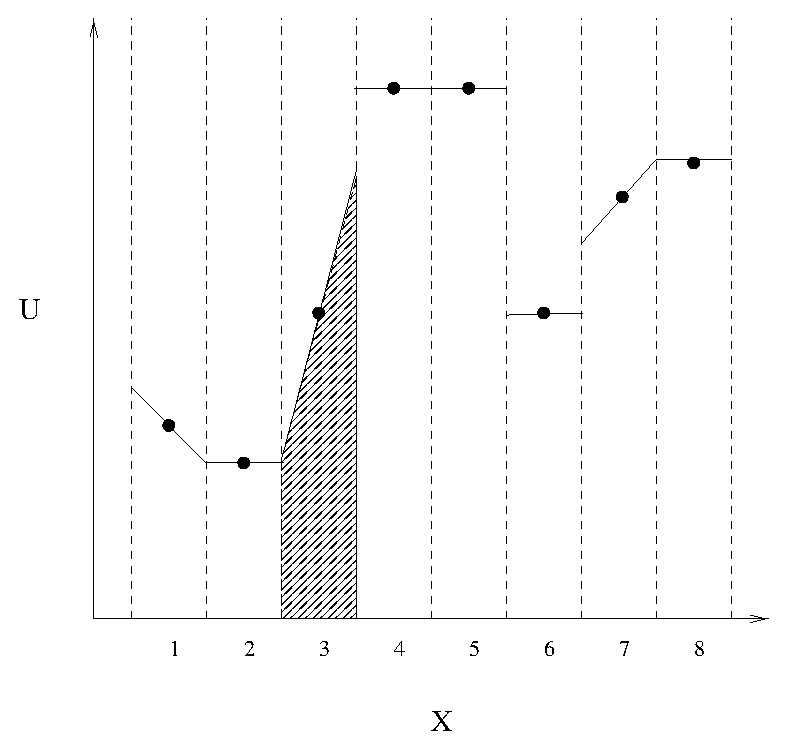
\epsfig{file=fivol.eps,height=7cm}}
   \caption{Finite volume representation of 1D data. The grid cells are
            bounded by cell interfaces (dashed lines).
            The dots represent the cell averages of $U$.
            The solid lines show possible extrapolations of $U$ to the
            cell interfaces.}
\label{fig:fivol}
\end{figure}

\BATSRUS\ uses a finite volume discretization of the MHD equations.
Space is divided into {\bf grid cells}, and the discrete conservative
variables are defined as the cell-averages 
\begin{equation}
   W_j(t) = \frac{1}{V_j}\int_{V_j} W(\bx,t) d\bx
\label{q-average}
\end{equation}
where $V_j$ is the volume of the cell indexed by $j$ (see Fig.~\ref{fig:fivol}).
The differential equations (\ref{q-compact}) are discretized in their 
integral form
\begin{equation}
   \frac{\partial W_j}{\partial t}=
     \frac{1}{V_j}\int_{V_j}\left(-\nabla\cdot \bF + S\right)\,d\bx
\label{q-integral}
\end{equation}
i.e. the equations are integrated for the cell volume. Using the Gauss
theorem, the volume integral of fluxes can be replaced by a surface integral.
In the discrete form we obtain
\begin{equation}
   W^{n+1}_j=W^n_j 
      -\frac{\Delta t}{V_j}\sum_{l=1}^{6}\bF^n_l\cdot\bn_l + \Delta t S_j^n
\label{q-fivol}
\end{equation}
where $\bF_l$ and $\bn_l$ are the flux and the normal surface vector
through the $l$-th face of cell $j$. The source term is simply evaluated
for $W_j^n$, which is a second order approximation to the volume averaged
source term. Second order time accuracy can be achieved by 
the two-stage scheme (\ref{q-two-stage}). 

The finite volume method automatically leads to a conservative 
discretization since the fluxes are defined at the cell interfaces and
they are added to and subtracted from the neighboring cell-averages
such that the total change remains zero. This argument holds when the
time step $\Delta t$ is the same for all the cells. 
For local time stepping, the conservation
is only ensured for the final steady state, when $W^{n+1}=W^n$ and thus
\begin{equation}
   \frac{1}{V_j}\sum_{l=1}^{6}\bF^n_l\cdot\bn_l = S_j^n
\label{q-fivol-steady}
\end{equation}
for each cell independent of the time step. An additional complication
arises for the AMR grid at resolution changes, where the face of a coarse cell
is shared with 4 fine cell neighbors. \BATSRUS\ ensures conservation 
by setting the flux for the coarse cell equal to the sum of the 4 fine fluxes.

The remaining question is how to calculate the fluxes at the cell faces.
\BATSRUS\ provides several numerical flux functions. These differ in their
diffusiveness and robustness. In general the more diffusive the scheme, 
the more robust it is. It is problem dependent which flux function should
be used. In principle one should select the least diffusive scheme which
is still robust enough to handle the problem. In practice it is difficult
to tell in advance whether a scheme will work or not for the full run,
so some experimentation may be required. In the following sections
we describe the available flux functions and slope limiters. 
For sake of concreteness we concentrate on the flux through the face
orthogonal to the $x$ direction.

\subsection{Roe flux \label{section:roe}}

The Roe flux is the most accurate, costly, and least robust of the three
available flux functions. It is based on an approximate solution of
the Riemann problem. The Riemann problem arises at the cell interface:
given the state vectors $W^L$ and $W^R$ on the left and right sides
of the interface, what will be the flux through the cell interface?

The Roe solver uses a characteristic decomposition of the discontinuity
$W^R-W^L$ to obtain an answer. The amplitude of the $k$-th characteristic wave
can be determined by multiplying the jump with the $k$-th left eigenvector
$l^k$ of the $\partial F/\partial W$ matrix. The $k$-th characteristic
wave moves with a speed $\lambda^k$. Depending on the sign of $\lambda^k$,
we should use the left or the right state to evaluate the flux.
After some algebra, the Roe flux is obtained
\begin{equation}
   F^{\rm Roe}_l = 
      \frac{F^R+F^L}{2} - \frac12 \sum_k r^k |\lambda^k| l^k (W^R-W^L)
\label{q-roe}
\end{equation}
where $r^k$ is the $k$-th right eigenvector of $\partial F/\partial W$. 
The eigenvectors and the eigenvalues are evaluated at some average state 
of $W^R$ and $W^L$.
We use the arithmetic average of the primitive variables $(U^R+U^L)/2$
for this purpose.

The Roe solver requires the calculation of the left and right eigenvectors 
and all the eigenvalues.
This is quite expensive for the MHD equations, although \BATSRUS\ uses a 
highly optimized subroutine for the flux calculation. The Roe solver is
not implemented for the Boris corrected MHD equations, because the eigenvectors
are too complicated. 

We mention that an entropy fix is implemented for the Roe flux, which
prevents the formation of rarefaction shock waves. The entropy fix
slightly increases $|\lambda^k|$ when it is very close to zero.

\subsection{Rusanov flux \label{section:rusanov}}

The Rusanov (also called TVD Lax-Friedrich or TVDLF) flux function greatly
simplifies the Roe solver by replacing $|\lambda^k|$ in (\ref{q-roe}) with 
\begin{equation}
\lambda^{\max}=\max_k |\lambda^k| = c_x + |u_x|
\end{equation}
where $c_x$ is the fast magnetosonic speed. Since now $\lambda^{\max}$ 
can be taken out of the sum and the product of left and right eigenvectors 
give a Kronecker delta in (\ref{q-roe}), the Rusanov flux function becomes
\begin{equation}
   F^{\rm Rusanov}_l = 
      \frac{F^R+F^L}{2} - \frac12 \lambda^{\max} (W^R-W^L)
\label{q-rusanov}
\end{equation}
Again, $\lambda^{\max}$ is evaluated for the average of primitive variables.
Note that the same $\lambda^{\max}$ is used for the time step calculation 
in (\ref{q-local-dt}). For cell $j$ we actually take the larger of
$\lambda_{j-1/2}^{\max}$ and $\lambda_{j+1/2}^{\max}$.

The Rusanov flux function is very efficient and robust, but more diffusive
than the Roe flux. Especially contact discontinuities diffuse fast for the
Rusanov flux function.

\subsection{Linde flux \label{section:linde}}

The Linde flux is in between the Roe and Rusanov fluxes in every sense.
It is more accurate but more expensive and less robust than the Rusanov flux, 
on the other hand, it is less accurate but less expensive and more robust
than the Roe-flux.

\subsection{First and Second Order Accuracy \label{section:order_accuracy}}

We still need to define how the left and right states $W^L$ and $W^R$ are
obtained. For a first order scheme
\begin{eqnarray}
W_{j+1/2}^L&=&W_{j}     \nonumber\\
W_{j+1/2}^R&=&W_{j+1}   \label{q-LR-first-order}
\end{eqnarray}
Spatially first order schemes are extremely diffusive, even for a Roe flux.
They should only be used at the very beginning of a steady state calculation,
since the first order schemes are fast and robust, so they can overcome
the initial transients. For the final steady state solution as well
as for a time accurate simulation, however, a spatially second order scheme 
is required. 

Second order spatial accuracy is achieved by a linear reconstruction
of the left and right states. To guarantee positivity, 
\BATSRUS\ uses the primitive variables $U=\{\rho,\bu,\bB,p\}$ 
for the linear reconstruction
\begin{eqnarray}
  U_{j+1/2}^L&=&U_{j}\ \ \ 
  + \frac{\Delta x}{2}\left(\frac{\partial U}{\partial x}\right)_j 
\nonumber\\
   U_{j+1/2}^R&=&U_{j+1} 
  - \frac{\Delta x}{2}\left(\frac{\partial U}{\partial x}\right)_j 
\label{q-LR-second-order}
\end{eqnarray}
The gradient $\partial V/\partial x$ must be carefully defined so that
no spurious oscillations are produced by the numerical scheme. 

\subsection{Slope Limiters \label{section:limiters}}

\begin{figure}
   \centerline{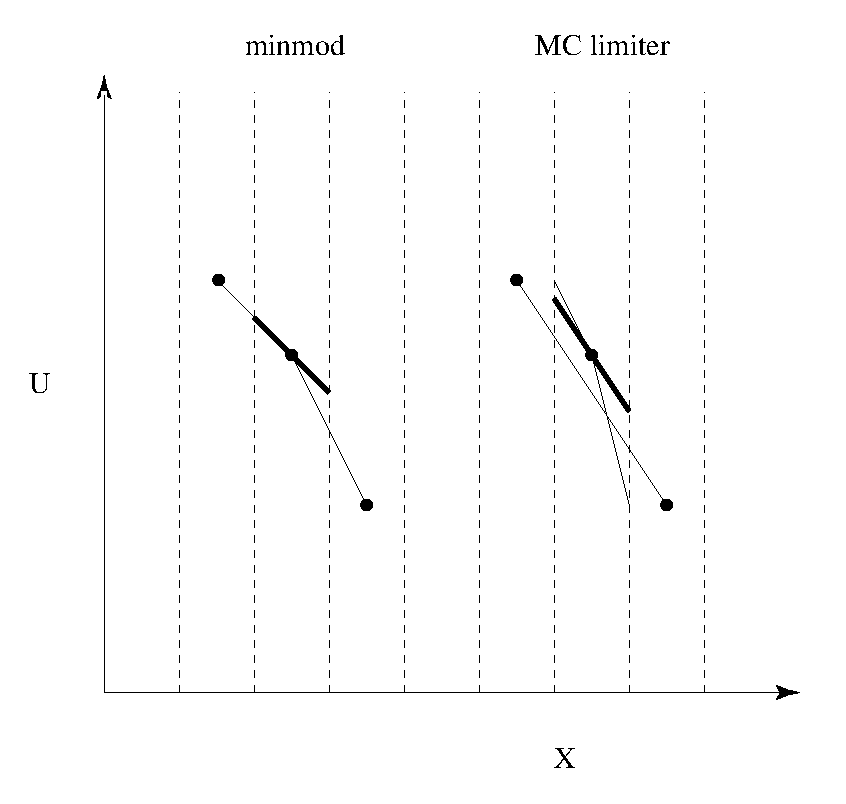
\epsfig{file=slope.eps,height=9cm}}
   \caption{Three different slope limiters applied to the same
            configuration. Each limiter considers a few different 
            approximate slopes (thin lines) and selects one of them
            (thick line).
           }
\label{fig:limiter}
\end{figure}

There are several possibilities to define oscillation free gradients. 
We implemented two variants in \BATSRUS: the {\bf minmod} limiter
and the {\bf monotonized central} (MC) limiter. The minmod limiter
is more diffusive and more robust, while the MC limiter is less diffusive
and less robust. The computational cost is very comparable, although the
minmod limiter is slightly less expensive.

The minmod and MC limited slopes are defined as
\begin{eqnarray}
   \left(\frac{\partial U}{\partial x}\right)^{\rm minmod}_j &=& 
   \frac{1}{\Delta x}\minmod\left(\DU_{j-1/2},\DU_{j+1/2}\right) 
\label{q-limiter} \\
   \left(\frac{\partial U}{\partial x}\right)^{\rm MC}_j~~~~ &=&
  \frac{2}{\Delta x}\minmod\left(\DU_{j-1/2},\DU_{j+1/2}, 
           \frac14(U_{j+1}-U_{j-1})\right)
\nonumber
\end{eqnarray}
where $\DU_{j+1/2}=U_{j+1}-U_j$ and the {\bf minmod} 
function is defined as the argument with the smallest modulus 
when all arguments have the same signs and otherwise it is zero.
The action of the slope limiters is depicted in Fig.~\ref{fig:limiter}.


%\end{document}



